%\section{Problem Definition}
\subsection{Similarity Search for Geolocated Time Series}
\label{sec:problem}

Next, we introduce our notation and define the distance functions for geolocated time series. Then, we outline different hybrid query variants, combining spatial distance with time series similarity.

\begin{table}[!t]
 \centering
 \caption{Hybrid query variants.}
 \vspace{-10pt}
 \begin{tabular}{c c c}
  \toprule
  Query Variant & Spatial Filter & Time Series Filter \\
  \midrule
  $Q_{bb}$ & boolean ($\theta_{sp}$) & boolean ($\theta_{ts}$) \\
  $Q_{kb}$ & top-$k$ & boolean ($\theta_{ts}$) \\
  $Q_{bk}$ & boolean ($\theta_{sp}$) & top-$k$ \\
  $Q_{hb}$ & \multicolumn{2}{c}{boolean ($\theta_{h}$)} \\
  $Q_{hk}$ & \multicolumn{2}{c}{top-$k$} \\
  \bottomrule
 \end{tabular}
 \label{tab:query_types}
\end{table}




\subsubsection{Preliminaries}
\label{subsec:preliminaries}
A {\em time series} is a time-ordered sequence of values $T = \{v_1, \ldots, v_w\}$, where $v_i$ is the value at the $i$-th time point and $w$ is the length of the series. In our work, each time series is also characterized by a location, denoted by $T.loc$. For brevity, in the sequel such {\em geolocated time series} will be also called objects. Assuming a 2-dimensional space, we further use the notation $T.loc_x$, $T.loc_y$ to refer to the $(x,y)$ coordinates of $T$'s location. Next, we define the {\em distance measures} we employ for similarity search on geolocated time series.

In the {\em spatial domain}, the distance between two geolocated time series $T$ and $T'$ is calculated using the Euclidean distance of their respective locations. Furthermore, we normalize this distance with $maxDist_{sp}$, i.e., the maximum spatial distance of any pair of objects in the dataset, to obtain a measure in the interval $[0,1]$. Thus:
\begin{equation} \label{eq:dist_sp}
 dist_{sp}(T, T') = \frac{\sqrt{(T.loc_x - T'.loc_x)^2 + (T.loc_y - T'.loc_y)^2}}{maxDist_{sp}}
\end{equation} \label{eq:2}

In the {\em time series domain}, similar to many prior works (e.g., \cite{shieh2008kdd}), we also apply the Euclidean distance to measure the similarity of a pair of objects. Specifically, we calculate the distance between two time series $T$ and $T'$ as follows:
\begin{equation} \label{eq:dist_ts}
 dist_{ts}(T, T') = \frac{\sqrt{\displaystyle \sum_{i=1}^{w}(v_i - v'_i)^2}}{maxDist_{ts}}
\end{equation}

\noindent where $maxDist_{ts}$ denotes the maximum distance of any pair of objects in the dataset and is used for normalization, as above.

Finally, we define a {\em hybrid distance} measure $dist_h(T, T')$ between two objects $T$ and $T'$, combining both their distances $dist_{sp}(T, T')$ in the spatial domain and $dist_{ts}(T, T')$ in the time series domain. For that purpose, we apply an {\em exponential decay} function to decrease the similarity of two time series based on their spatial distance:
\begin{equation}
 sim_h(T, T') = sim_{ts}(T, T') \; e^{- \gamma \; dist_{sp}(T, T')}
 \label{eq:sim_h}
\end{equation}

\noindent where $sim_{ts}(T, T') = 1 - dist_{ts}(T, T')$ and $\gamma$ is the exponential decay constant. Then:
\begin{equation}
 dist_h(T, T') = 1 - sim_h(T, T')
 \label{eq:dist_h}
\end{equation}

Accordingly, the hybrid similarity (distance) between two objects $T$ and $T'$ is equal to their standard time series similarity (distance) if they are located at the same position, and it gradually decreases (respectively, increases) if one is placed farther apart from the other.

%Finally, we combine the two above distance functions to obtain a hybrid distance measure for geo-located time-series as follows:
%\begin{equation} \label{eq:4}
% dist_h(T, T') = \lambda \cdot \frac{dist_{sp}(T, T')}{maxD_{sp}} + (1 - \lambda) \cdot \frac{dist_{ts}(T, T')}{maxD_{ts}}
%\end{equation}
%where $maxD_{sp}$ and $maxD_{ts}$ refer to the maximum distance in the spatial and time-series domain respectively and are used for normalization and $\lambda \in [0,1]$ is a weighting parameter determining the relative importance of each individual distance measure.



\subsubsection{Hybrid Query Variants}
\label{subsec:query_types}


\begin{figure}[!t]
 \centering
 \subfloat[$Q_{bb}(T_q, \theta_{sp}, \theta_{ts})$]{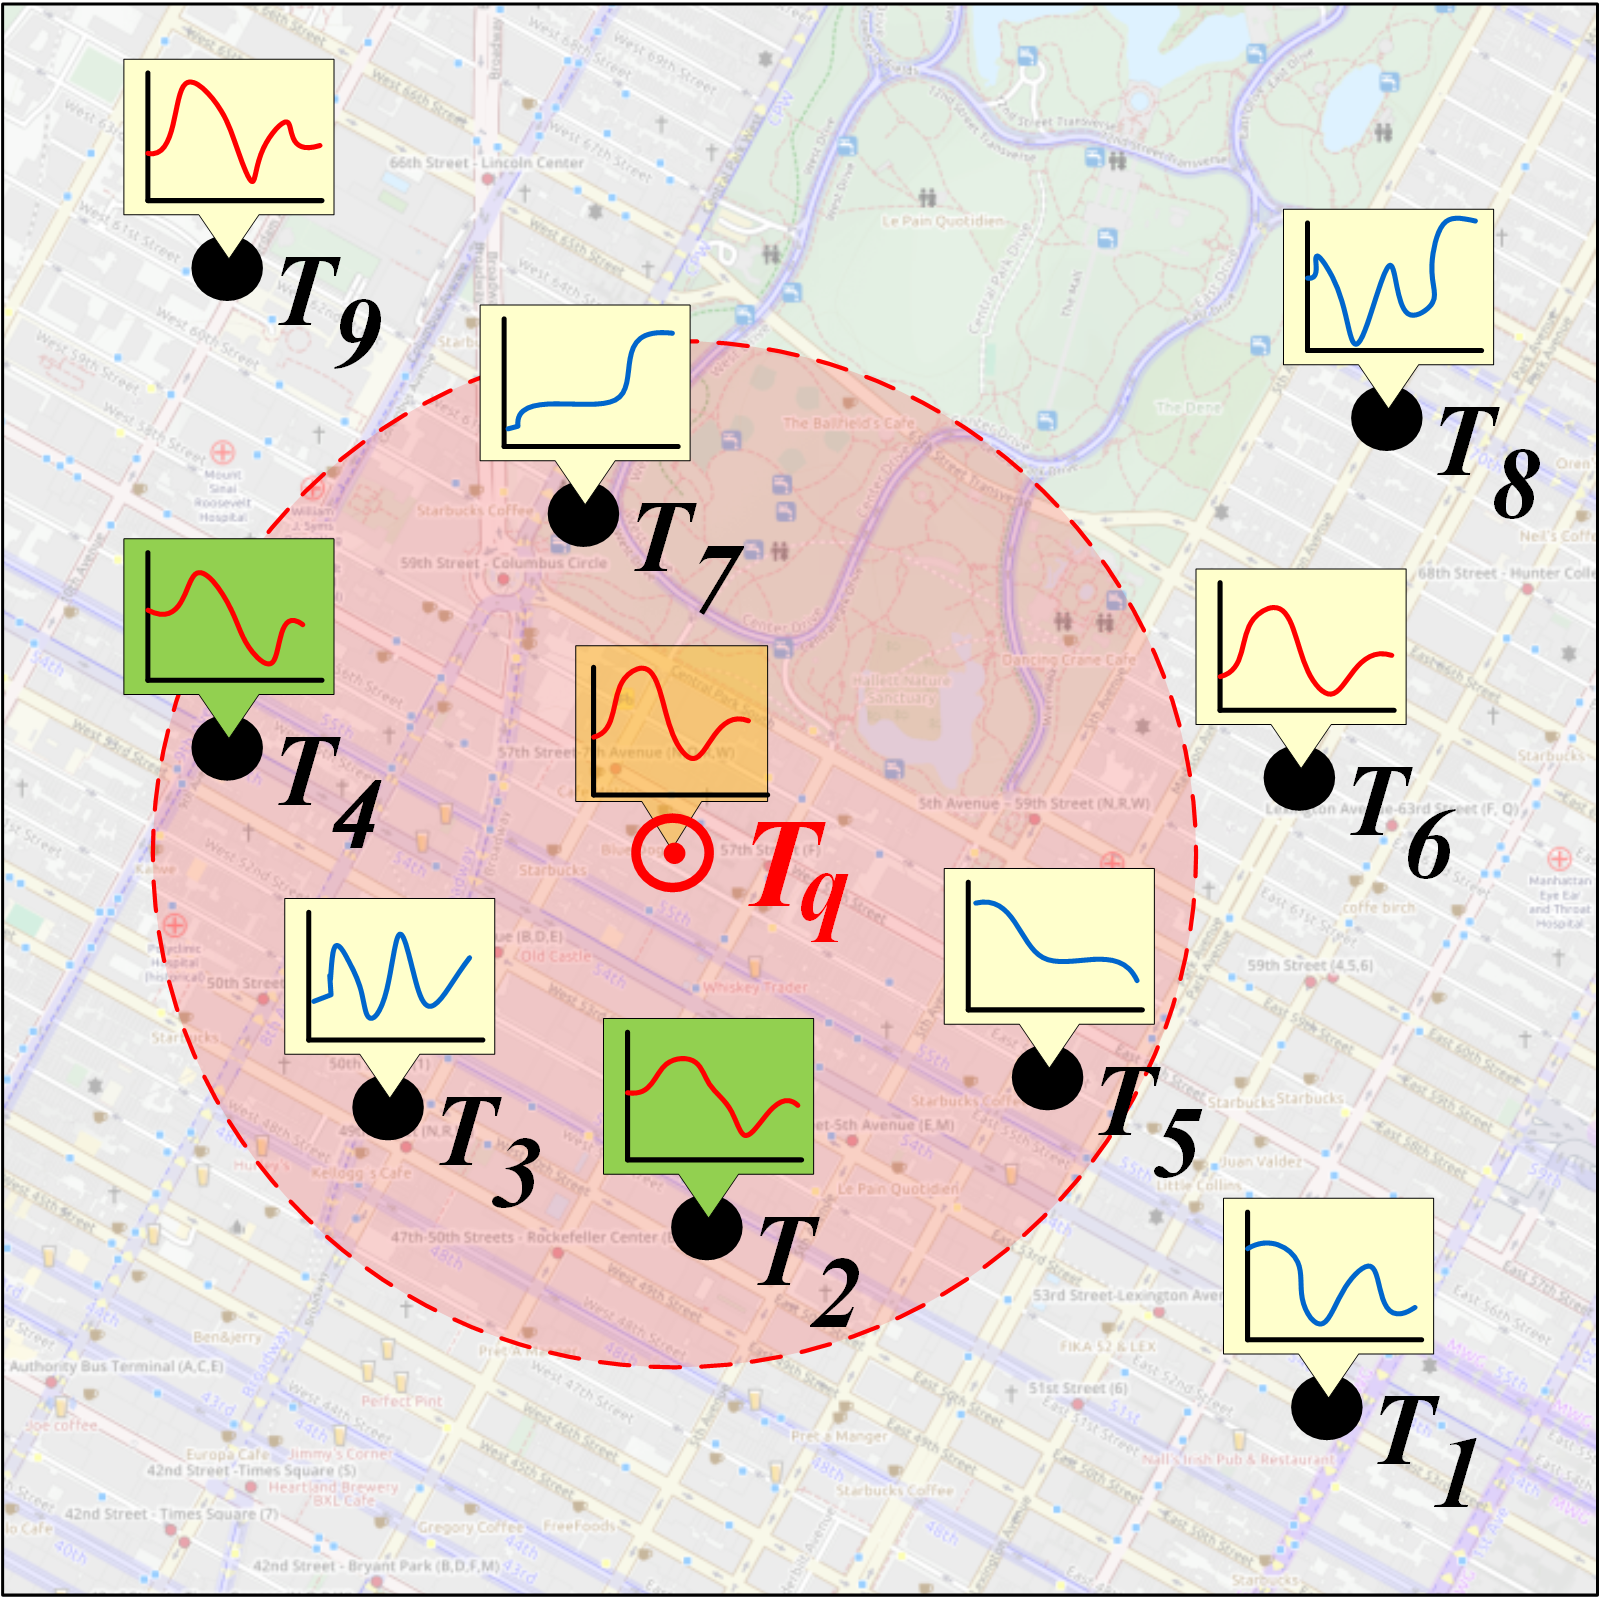
\includegraphics[width=0.23\textwidth]{figures/query_bb.png}\label{subfig:example_queries_bb}}
 \subfloat[$Q_{kb}(T_q, k, \theta_{ts})$]{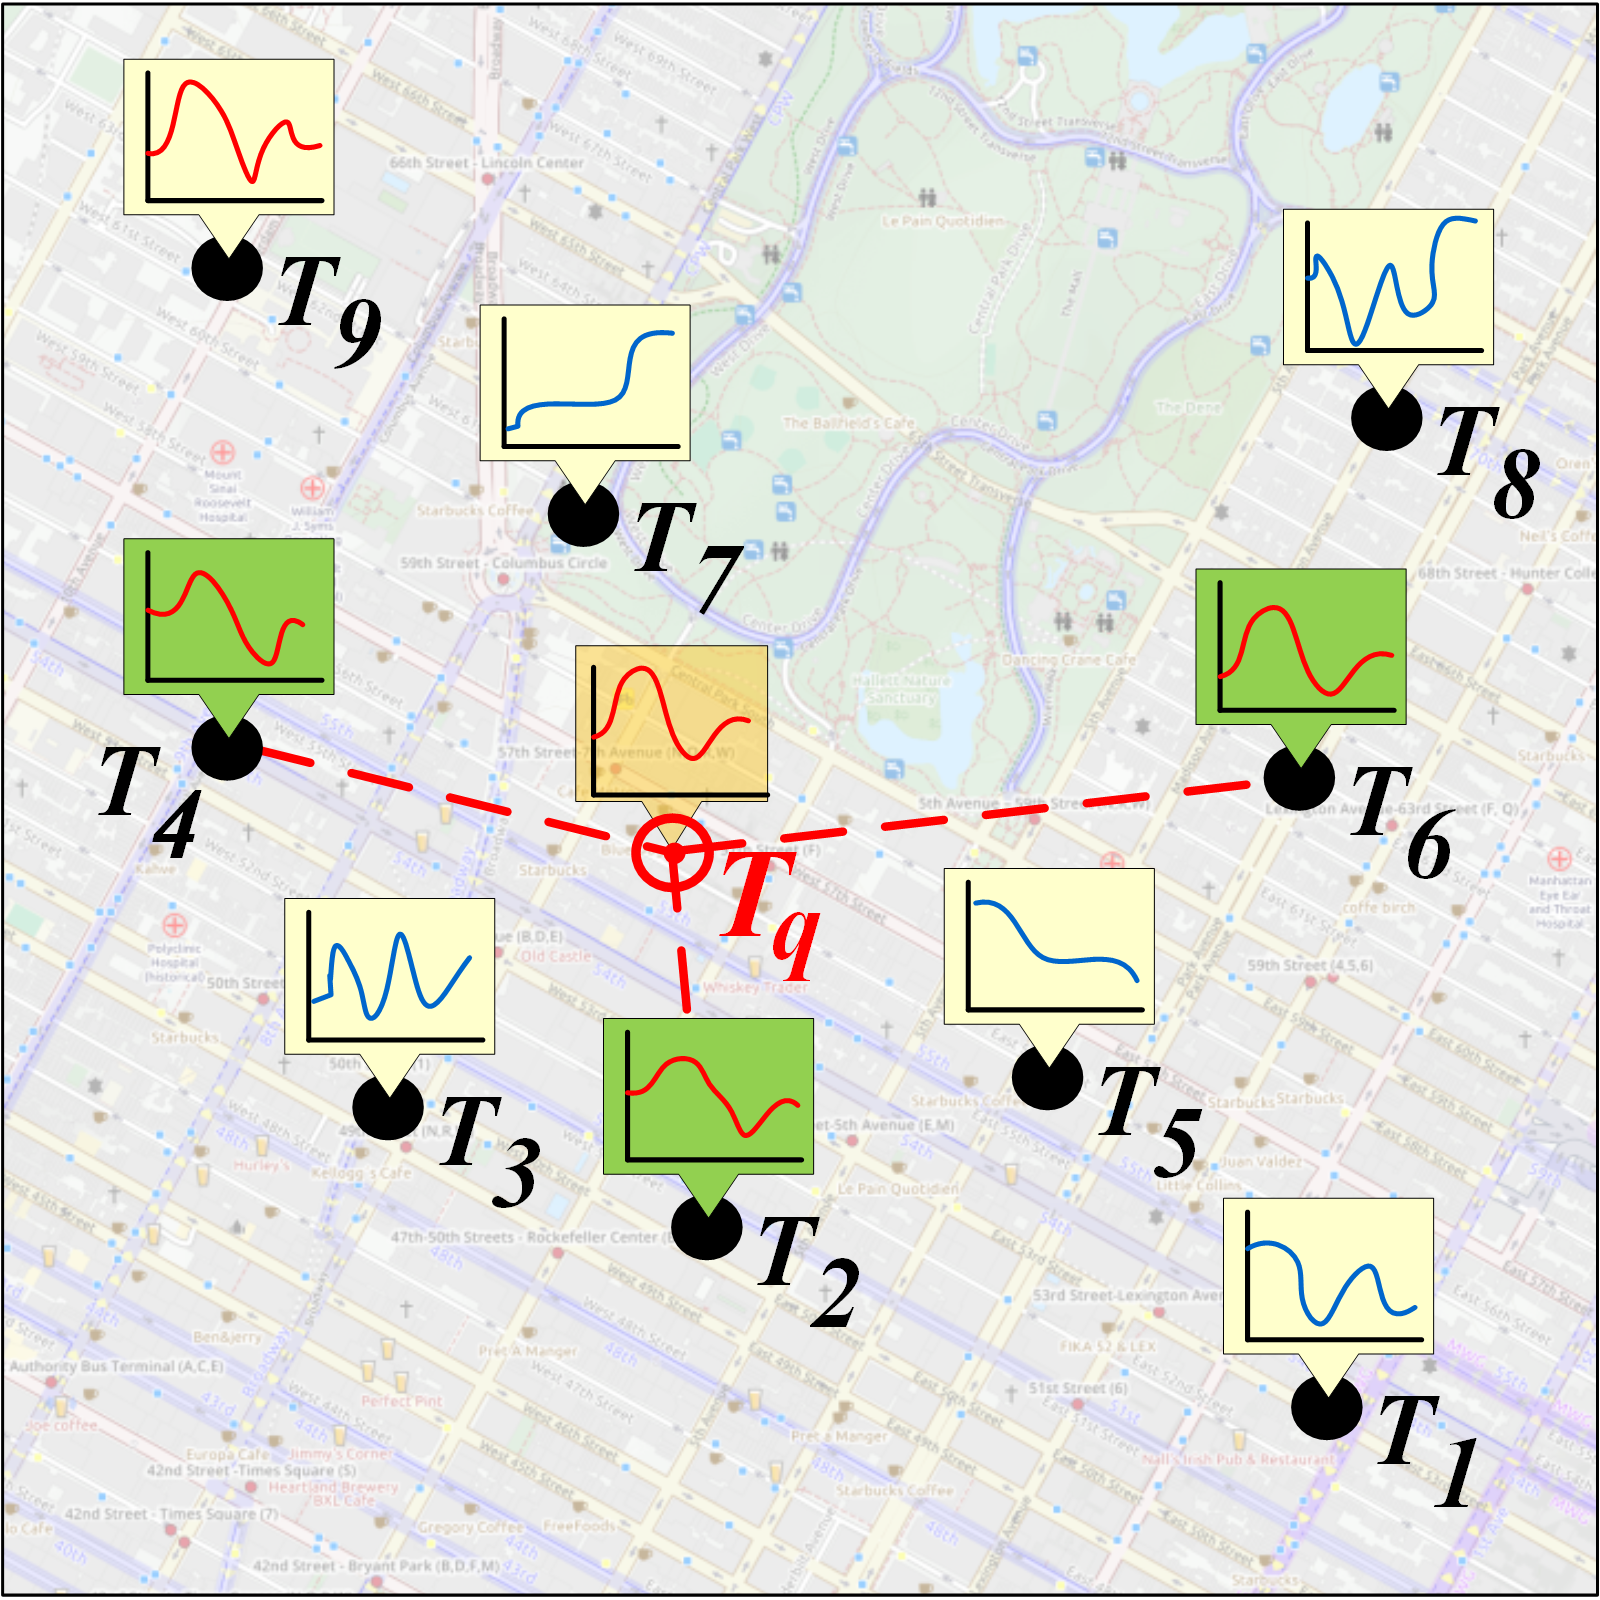
\includegraphics[width=0.23\textwidth]{figures/query_kb.png}\label{subfig:example_queries_kb}}
\caption{Hybrid queries on geolocated time series.}
\label{fig:example_queries}
\end{figure}


We are interested in {\em hybrid queries} on geolocated time series, i.e., queries that retrieve search results based on both spatial distance and time series distance. In these queries, a geolocated time series $T_q$ is given as a reference, and the goal is to identify similar time series to $T_q$, based on both spatial distance and time series distance.


Different query variants can be derived. First, the query condition can be applied on each distance independently or on the hybrid distance defined above. Second, the condition can be a boolean filter (i.e., retrieve all objects with distance lower than $\theta$) or a top-$k$ filter (i.e., retrieve the $k$ objects having the smallest distance). These lead to the query variants listed in Table \ref{tab:query_types} and outlined below:


\begin{itemize}
 \item $Q_{bb}(T_q, \theta_{sp}, \theta_{ts})$. This query applies two individual boolean filters. It retrieves each time series $T$ having $dist_{sp}(T_q, T) \leq \theta_{sp}$ and $dist_{ts}(T_q, T) \leq \theta_{ts}$. In other words, it retrieves all time series that are located within a radius $\theta_{sp} \cdot maxDist_{sp}$ from $T_q$'s location and their time series dissimilarity to $T_q$ is at most $\theta_{ts} \cdot maxDist_{ts}$.
 \item $Q_{kb}(T_q, k, \theta_{ts})$. This query retrieves the $k$ time series closest to $T_q$'s location also having $dist_{ts}(T_q, T) \leq \theta_{ts}$.
 \item $Q_{bk}(T_q, \theta_{sp}, k)$. This query retrieves the $k$ most similar time series to $T_q$ which are also located within distance $\theta_{sp} \cdot maxDist_{sp}$ from $T_q$'s location.
 \item $Q_{hb}(T_q, \theta_h, \gamma)$. This query retrieves all time series having hybrid distance to $T_q$ at most $\theta_h$, i.e., $dist_h(T_q, T) \leq \theta_h$.
 \item $Q_{hk}(T_q, k, \gamma)$. This query retrieves the $k$ time series with the smallest hybrid distance $dist_h(T_q, T)$ to $T_q$.
\end{itemize}




\begin{figure*}[!t]
 \centering
 \subfloat[MBTS in \tsr]{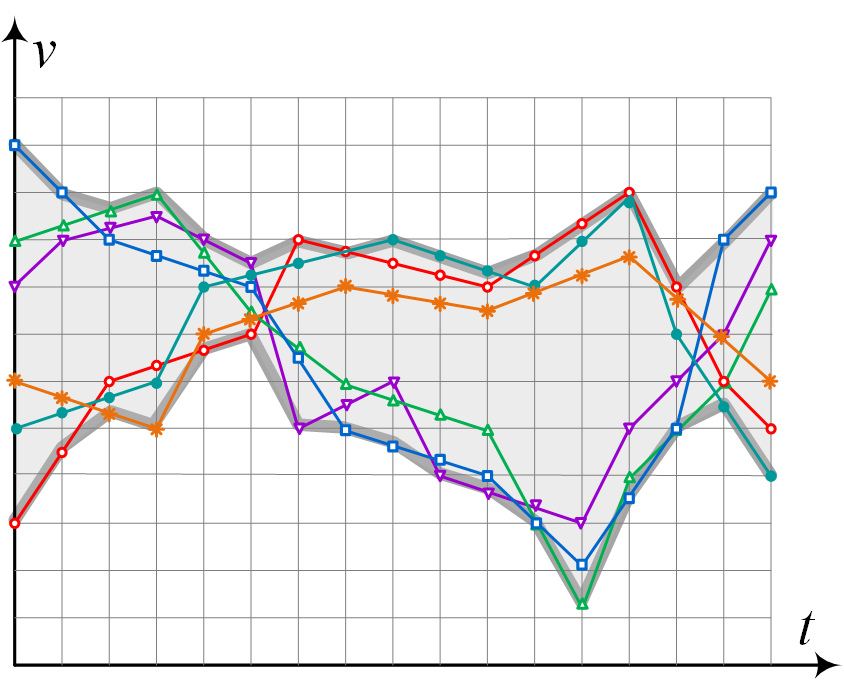
\includegraphics[width=0.32\textwidth]{figures/bounds_tsr.png}\label{subfig:tsr_mbts}}\hspace{8pt}
 \subfloat[Distance bounds with MBTS]{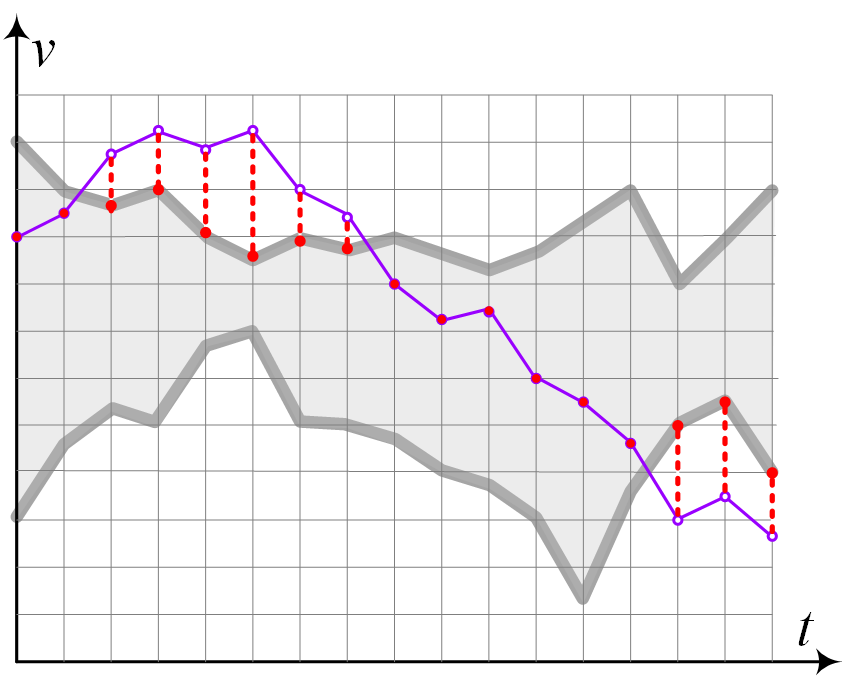
\includegraphics[width=0.32\textwidth]{figures/bounds_mindst.png}\label{subfig:mbts_bounds}}\hspace{8pt}
 \subfloat[MBTS in \ctsr]{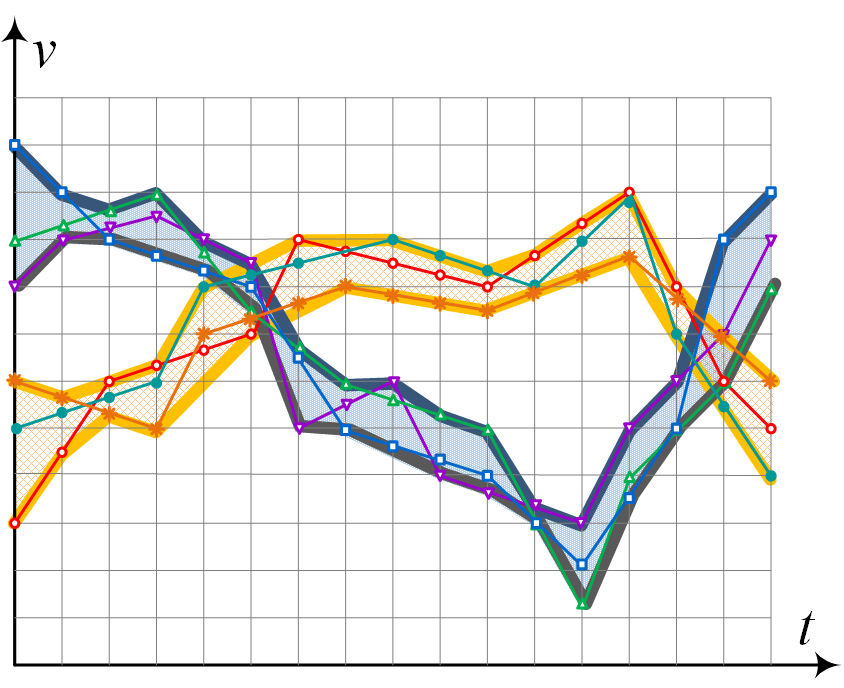
\includegraphics[width=0.32\textwidth]{figures/bounds_ctsr.png}\label{subfig:btsr_mbts}}
\caption{Examples illustrating the time series bounds and pruning in \tsr and \ctsr.}
\label{fig:example_bounds}
\end{figure*}


\begin{myexample}
 Figure \ref{fig:example_queries} illustrates an example including two hybrid queries, $Q_{bb}(T_q, \theta_{sp}, \theta_{ts})$ and $Q_{kb}(T_q, k, \theta_{ts})$, on a set of geolocated time series $T_1$, \ldots, $T_9$. In both cases, the reference time series $T_q$ specified by the query is shown in red. Moreover, those time series having dissimilarity to $T_q$ at most $\theta_{ts}$ (i.e., $T_2$, $T_4$, $T_6$, $T_9$) are also shown with red lines. In the first query, only time series within a radius equal to the spatial distance threshold $\theta_{sp}$ are retrieved. Thus, the result contains only time series $T_2$ and $T_4$, whereas $T_6$ and $T_9$ are excluded. The second query for $k=3$ retrieves the three closest time series to $T_q$ having dissimilarity at most $\theta_{ts}$, i.e., $T_2$, $T_4$ and $T_6$. \qed
\end{myexample}